% !TEX program = xelatex
\documentclass[a4paper,8pt]{article}

% 中文字体
\usepackage{xeCJK}
%\setmainfont{Times New Roman}
\setmainfont{Arial}
%\setCJKmainfont{WenQuanYi Micro Hei}
\setCJKmainfont{Microsoft YaHei}
% 段首缩进
\usepackage{indentfirst}
% 数学符号
\usepackage{amsfonts} 
\usepackage{amsmath}
% 代码块
\usepackage{listings}
\usepackage{xcolor}
\lstset{numbers=left, %设置行号位置
basicstyle=\footnotesize, % 代码字号
numberstyle=\tiny, %设置行号大小
keywordstyle=\color{blue}, %设置关键字颜色
commentstyle=\color[cmyk]{1,0,1,0}, %设置注释颜色
frame=single, %设置边框格式
escapeinside=``, %逃逸字符(1左面的键),用于显示中文
breaklines, %自动折行
extendedchars=false, %解决代码跨页时,章节标题,页眉等汉字不显示的问题
xleftmargin=2em,xrightmargin=2em, aboveskip=1em, %设置边距
tabsize=4, %设置tab空格数
showspaces=false %不显示空格
}
% 图片
\usepackage{graphicx}
\usepackage{subfigure}
% 斜线表头
\usepackage{diagbox}


% 姓名
\author{22035036 刘明}
% 题目
\title{感知机模型理论及编程实验}
% 页眉
\pagestyle{headings}

% 正文
\begin{document}

\maketitle

\tableofcontents

\newpage

\section{感知机模型的简介和历史}
\label{sec:introduction}
\subsection{简介}
感知机(英语:Perceptron)是Frank Rosenblatt在1957年就职于康奈尔航空实验室(Cornell Aeronautical Laboratory)时所发明的一种人工神经网路。它可以被视为一种最简单形式的前馈神经网路,是一种二元线性分类器。

Frank Rosenblatt给出了相应的感知机学习算法,常用的有感知机学习,最小二乘法和梯度下降法。譬如,感知机利用梯度下降法对损失函数进行极小化,求出可将训练数据进行线性划分的分离超平面,
从而求得感知机模型。

感知机是生物神经细胞的简单抽象。神经细胞结构大致可分为:树突,突触,细胞体及轴突,如图 \ref{fig:neuron}。单个神经细胞可被视为一种只有两种状态的机器——激动时为“是”,而未激动时为“否”。神经细胞的状态取决于从其它的神经细胞收到的输入信号量,及突触的强度(抑制或加强)。当信号量总和超过了某个阈值时,细胞体就会激动,产生电脉冲。电脉冲沿着轴突并通过突触传递到其它神经元。为了模拟神经细胞行为,与之对应的感知机基础概念被提出,如权量(突触),偏置(阈值)及激活函数(细胞体)。

\begin{figure}[htbp]
\centering
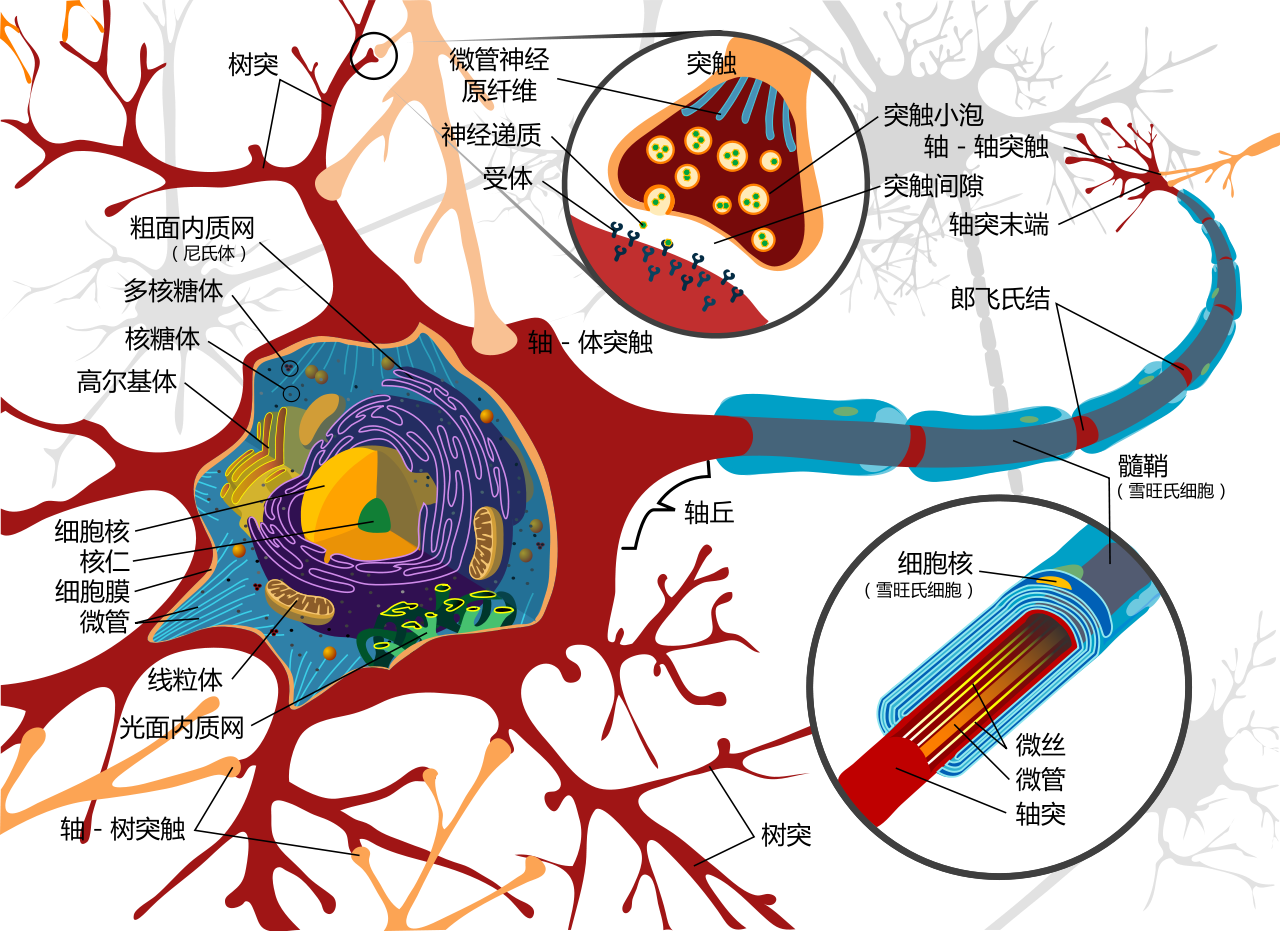
\includegraphics[width=10cm]{./fig/神经细胞结构图.png}
\caption{ 神经细胞结构图}\label{fig:neuron}
\end{figure}

在人工神经网络领域中,感知机也被指为单层的人工神经网络,以区别于较复杂的多层感知机(Multilayer Perceptron)。作为一种线性分类器,(单层)感知机可说是最简单的前向人工神经网络形式。尽管结构简单,感知机能够学习并解决相当复杂的问题。感知机主要的本质缺陷是它不能处理线性不可分问题。

\subsection{历史}
1943年,心理学家沃伦·麦卡洛克和数理逻辑学家沃尔特·皮茨在合作的《A logical calculus of the ideas immanent in nervous activity》论文中提出并给出了人工神经网络的概念及人工神经元的数学模型,从而开创了人工神经网络研究的时代。1949年,心理学家唐纳德·赫布在《The Organization of Behavior》论文中描述了神经元学习法则——赫布型学习。

人工神经网络更进一步被美国神经学家弗兰克·罗森布拉特所发展。他提出了可以模拟人类感知能力的机器,并称之为“感知机”。1957年,在Cornell航空实验室中,,他成功在IBM 704机上完成了感知机的仿真。两年后,他又成功实现了能够识别一些英文字母,基于感知机的神经计算机——Mark1,并于1960年6月23日,展示与众。

为了“教导”感知机识别图像,弗兰克·罗森布拉特在Hebb学习法则的基础上,发展了一种迭代,试错,类似于人类学习过程的学习算法——感知机学习。除了能够识别出现较多次的字母,感知机也能对不同书写方式的字母图像进行概括和归纳。但是,由于本身的局限,感知机除了那些包含在训练集里的图像以外,不能对受干扰(半遮蔽,不同大小,平移,旋转)的字母图像进行可靠的识别。

首个有关感知机的成果,由弗兰克·罗森布拉特于1958年发表在《The Perceptron: A Probabilistic Model for Information Storage and Organization in the Brain》的文章里。1962年,他又出版了《Principles of Neurodynamics: Perceptrons and the theory of brain mechanisms》一书,向大众深入解释感知机的理论知识及背景假设。此书介绍了一些重要的概念及定理证明,例如感知机收敛定理。

虽然最初被认为有着良好的发展潜能,但感知机最终被证明不能处理诸多的模式识别问题。1969年,马文·明斯基和西摩尔·派普特在《Perceptrons》书中,仔细分析了以感知机为代表的单层神经网络系统的功能及局限,证明感知机不能解决简单的异或(XOR)等线性不可分问题,但弗兰克·罗森布拉特和马文·明斯基和西摩尔·派普特等人在当时已经了解到多层神经网络能够解决线性不可分的问题。

由于弗兰克·罗森布拉特等人没能够及时推广感知机学习算法到多层神经网络上,又由于《Perceptrons》在研究领域中的巨大影响,及人们对书中论点的误解,造成了人工神经领域发展的长年停滞及低潮,直到人们认识到多层感知机没有单层感知机固有的缺陷及反向传播算法在80年代的提出,才有所恢复。1987年,书中的错误得到了校正,并更名再版为《Perceptrons - Expanded Edition》。

近年,在Freund及Schapire(1998)使用核技巧改进感知机学习算法之后,愈来愈多的人对感知机学习算法产生兴趣。后来的研究表明除了二元分类,感知机也能应用在较复杂,被称为structured learning类型的任务上(Collins, 2002)。又或使用在分布式计算环境中的大规模机器学习问题上(McDonald, Hall and Mann, 2011)。

\section{模型和算法}

\subsection{线性可分概念}
线性可分的定义:对于数据集$T$,若存在超平面$S$能完全正确的将正例和反例划分在超平面两侧,则称$T$是线性可分的;否则称为线性不可分。

线性可分的判别方法:对两类数据点分别作凸包,若两个凸包不相交则是线性可分的,反之非线性可分。

高效的作出凸包并判断是否相交有许多算法,不过本文不需要深入探究,只需了解线性可分概念即可。

\subsection{感知机模型}
假设输入空间是$\mathcal{X} \subseteq \mathbb{R}^n$,输出空间是$ \mathcal{Y} = \{ +1,-1 \}$。输入$x\in \mathcal{X}$表示实例的特征向量,对应于输入空间的点,输出$y\in \mathcal{Y}$表示实例的类别。

感知机模型如下:
\begin{eqnarray}
f(x) = sign(w^T x + b)
\end{eqnarray}

其中,$w$和$b$为感知机模型参数,$w\in \mathbb{R}^n$叫做权值(weight)或权向量(weight vector),$b\in \mathbb{R}$为偏置(bias),$sign$为符号函数。

假设空间:所有线性分类模型。

几何解释:使用超平面$w^Tx+b=0$将特征空间划分为两个部分,分别为正反两类。

可以证明,对于线性可分的数据集,算法最终一定可以在有限次内收敛,即确定模型参数$w$和$b$,且收敛结果使所有的点都正确分类。具体证明参看第 \ref{sec:proof} 节。

对于线性不可分的情况,可以参考第 \ref{sec:extension} 节中的推广算法。

\subsection{最优化问题/损失函数}

按照我们的目的,是所有的点都正确分类,即
\begin{eqnarray}
y_i (w^T x_i +b) > 0 ,\forall i
\end{eqnarray}

因此,目标是错误分类数最小,最优化问题为
\begin{eqnarray}
\min \sum_i Error\left(y_i (w^T x_i +b)\right)
\end{eqnarray}

其中
\begin{eqnarray}
Error(x) =  
\begin{cases}
0 & x>0\\
1 & \text{otherwise}.
\end{cases}
\end{eqnarray}

但是这个目标函数不可导,不易优化。
因此,将目标改为错误分类点到超平面的距离之和最小,即
\begin{eqnarray}
\min \sum_{x_i \in M} -\frac{1}{\| w \|_2} y_i ( w^T x_i + b)
\end{eqnarray}

其中$M$为误分类点集合。

如果对当前问题使用梯度方法设计迭代格式,分母$\|w\|_2$会使得运算比较复杂。而由于我们的条件是数据集是线性可分的,也就是说如果我们达到了预期,找到了能完全正确划分数据点的超平面,则此时目标函数的值应为0,与分母$\|w\|_2$无关。因此,可以做适当的简化,将分母去掉,得到最终的目标:
\begin{eqnarray}
\min -\sum_{x_i \in M} y_i ( w^T x_i + b)
\end{eqnarray}

即,损失函数
\begin{eqnarray}
L(w,b) = -\sum_{x_i \in M} y_i ( w^T x_i + b)
\end{eqnarray}

此时,损失函数是一个连续可导函数,并且其偏导数的结构也很简单,易于计算。

\subsection{计算方法/学习算法}

最优化问题是一个无条件约束的问题,目标函数可导,最直接的方法就是梯度下降法(gradient descent,DG)。

当误分类点集合$M$固定时,损失函数的梯度为
\begin{eqnarray}
\nabla_w L = -\sum_{x_i\in M} y_i x_i  \\
\nabla_b L = -\sum_{x_i\in M} y_i
\end{eqnarray}

但是由于集合$M$的判别比较麻烦,比较难使用所有数据进行梯度下降。因此感知机模型通常采用随机梯度下降法(stochastic gradient descent,SDG),每次迭代时随机选择一个误分类点$x_i \in M$,对这个点使用梯度下降法进行更新:
\begin{eqnarray}
w & \leftarrow & w + \eta y_i x_i \\
b & \leftarrow & b + \eta y_i
\end{eqnarray}
其中$\eta(0< \eta\le 1)$在最优化问题中称为步长,在机器学习中称为学习率。直到没有误分类点,迭代终止,得到最优化问题的解,也就是能完全正确划分的超平面的参数$w^*$和$b^*$。

因为$w^T x + b = [w;b]^T [x;1]$,为了书写简单,我们使用$w$代指$[w;b]$,使用$x$代指$[x;1]$,此时,算法改写为
\begin{eqnarray}
w \leftarrow w + \eta y_i x_i
\end{eqnarray}

\section{收敛性证明}
\label{sec:proof}

在迭代过程中,每次遇到错误的点就修正,直到全部都正确为止。这种做法的思想是“知错能改”,有句话形容它:“A fault confessed is half redressed.”

在修正的过程中,之前分类正确的点可能变成错误的点,但我们能证明,对于线性可分的数据集,算法最终一定可以在有限次内收敛,且收敛结果使所有的点都正确分类。

当然,由于算法的终止条件是所有点都正确分类,那么如果数据本身是线性不可分的,那就迭代过程就永远无法终止了。在此我们仅讨论线性可分的数据,对于线性不可分的数据的处理方法参考第\ref{sec:extension}节。

下面给出证明。

根据线性可分定义,对于线性可分的情况,一定存在一个超平面$w_f$,满足
\begin{eqnarray}
y_i w_f^T x_i \ge \min_j y_j w_f^T x_j > 0, \quad \forall i
\end{eqnarray}

为简化书写,以下所有的范数$\|\cdot\|$均表示二范数$\|\cdot\|_2$。

为方便证明,我们还要求$\|w_f\|=1$,标准化即可。

使用$t$表示迭代次数。
使用$x_{n(t)}$表示第$t$次迭代时选中的错误分类点。
因为是错误分类点所以满足
\begin{eqnarray}
y_{n(t)} w_t^T x_{n(t)} \le 0
\end{eqnarray}

为了证明方便。取初始值$w_0=\vec{0}$,$w_t$表示第$t$次迭代后的$w$,
则有
\begin{eqnarray}
w_f^T w_t & = & w_f^T (w_{t-1} + \eta y_{n(t-1)} x_{n(t-1)}) \\
& = & w_f^T w_{t-1} + \eta y_{n(t-1)} w_f^T x_{n(t-1)} \\
& \ge & w_f^T w_{t-1} + \eta \min_j y_j w_f^T x_j \\
& \ge & w_f^T w_{0} + t \eta \min_j y_j w_f^T x_j \\
& = & t \eta \min_j y_j w_f^T x_j
\end{eqnarray}

且
\begin{eqnarray}
\|w_t\|^2 & = & \| w_{t-1} + \eta y_{n(t-1)} x_{n(t-1)} \|^2 \\
& = & \| w_{t-1}\|^2 + 2\eta y_{n(t-1)} w_t^T x_{n(t-1)}
+ \| \eta y_{n(t-1)} x_{n(t-1)} \|^2 \\
& \le & \| w_{t-1}\|^2 + 0 + \eta^2 \| x_{n(t-1)} \|^2 \\
& \le & \| w_{t-1}\|^2 + \eta^2 \max_j \| x_j \|^2 \\
& \le & \|w_0\|^2 + t \eta^2 \max_j \| x_j \|^2 \\
& = &  t \eta^2 \max_j \| x_j \|^2
\end{eqnarray}

得
\begin{eqnarray}
t \eta \min_j y_j w_f^T x_j \le w_f^T w_t \le \|w_f\| \|w_t\| \le \sqrt{t} \eta \max_j \| x_j \|
\end{eqnarray}

于是
\begin{eqnarray}
t \le \left( \frac{\max_j \| x_j \|}{\min_j y_j w_f^T x_j} \right)^2 \label{eqn:maxt}
\end{eqnarray}

因此,随着迭代次数增加,$w_t$越来越接近$w_f$,且误分类次数$t$有上界,即迭代会在有限次终止。

\section{编程实现和实验统计}

感知机算法的python代码可查看附录 \ref{sec:pythoncode}。

下面取20个随机的2维数据点和随机的$w_f$。给出一个迭代过程的例子,如图Figure \ref{fig:demo}。代码实现见$perceptron\_draw.py$。

\begin{figure}[htbp]
\centering
\subfigure[初始化$w_0 = (0,0,0)^T $]{
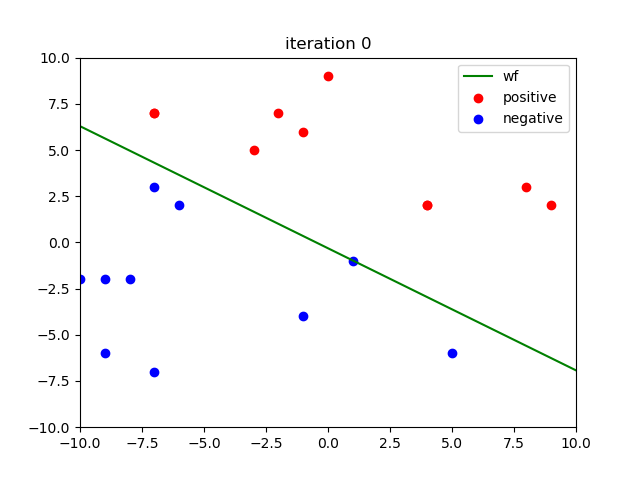
\includegraphics[width=5cm]{./fig/iter0.png}
}
\subfigure[第1次迭代$w_1$]{
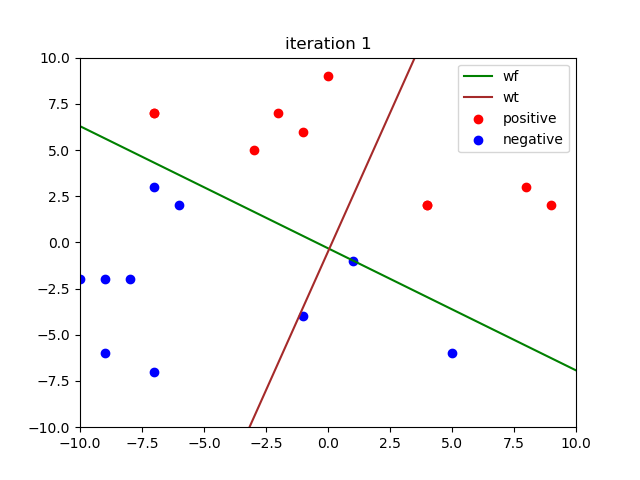
\includegraphics[width=5cm]{./fig/iter1.png}
}
\subfigure[第2次迭代$w_2$]{
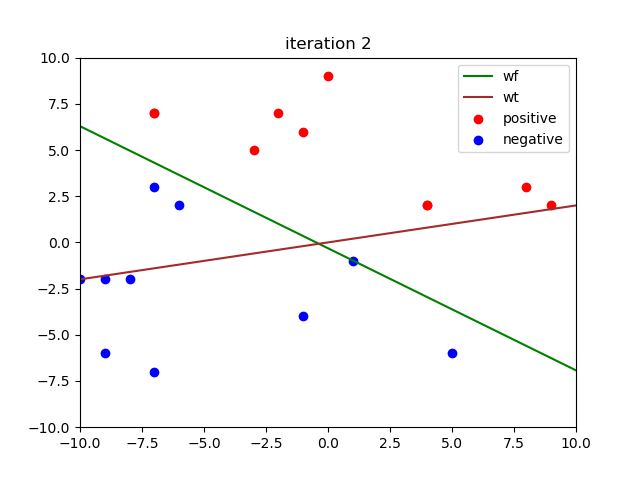
\includegraphics[width=5cm]{./fig/iter2.png}
}
\subfigure[第3次迭代$w_3$]{
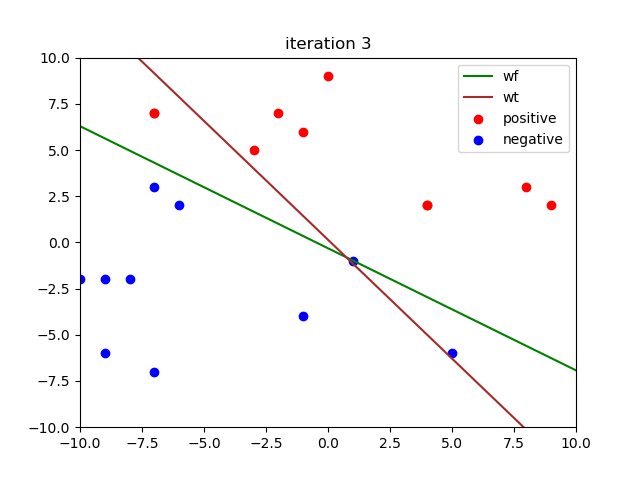
\includegraphics[width=5cm]{./fig/iter3.png}
}
\subfigure[第4次迭代$w_4$]{
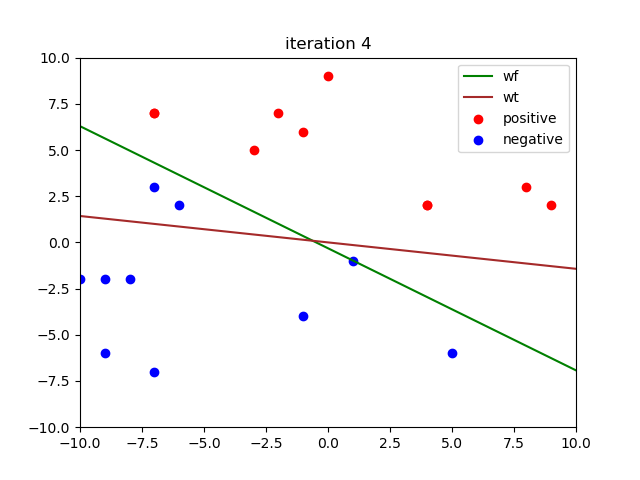
\includegraphics[width=5cm]{./fig/iter4.png}
}
\subfigure[第5次迭代$w_5$,终止]{
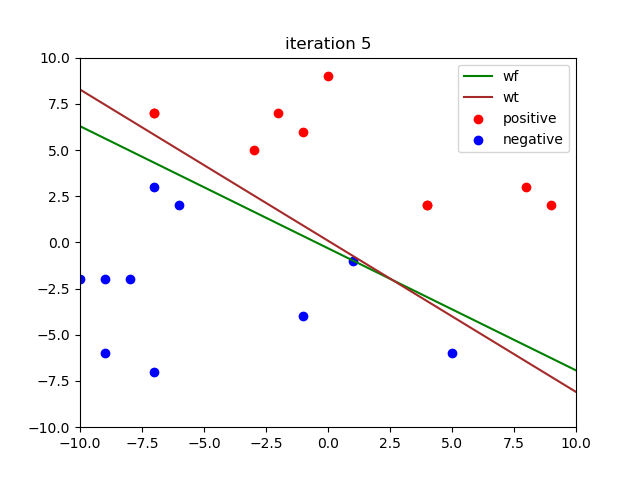
\includegraphics[width=5cm]{./fig/iter5.png}
}
\caption{ 感知机迭代过程示意图}\label{fig:demo}
\end{figure}

为了验证实际收敛次数的分布及其与我们在公式\ref{eqn:maxt}给出的最大收敛次数的关系,进行数值实验。代码实现见$perceptron\_stats.py$。

为了书写简单,令$t$表示实际迭代次数,$T$表示 \ref{eqn:maxt}给出的最大收敛次数,即
\begin{eqnarray}
T := \left( \frac{\max_j \| x_j \|}{\min_j y_j w_f^T x_j} \right)^2
\end{eqnarray}

\subsection{实验:实际迭代次数$t$和最大迭代次数$T$的大致取值}

经过几次数值实验,就可发现$t$是明显小于$T$的。

于是,本文通过重复实验取平均数来探究对于不同的样本总量和样本维数,$t$和$T$的大概取值。

结果见表 \ref{table:stats} ,结果为10000次实验的平均数,仅供参考。

\begin{table}[!htbp]
\centering
\begin{tabular}{|c|c|c|c|}
\hline
\diagbox{样本维数}{$\overline{t}/\overline{T}$}{样本总数}
&                 20 &                       100 &               1000 \\
\hline
2        &8.12/979.62&35.45/3570.38&110.77/11073.76\\
\hline
10     &7.93/1620.37&53.25/11906.91&1860.63/71941.19\\
\hline
100   &5.59/10018.35&27.57/51427.60&413.87/533825.22\\
\hline
1000   &1.34/8352.42&2.65/37908.47&18.32/332347.42\\
\hline
\end{tabular}
\caption{$\overline{t}/\overline{T}$统计表}
\label{table:stats}
\end{table}

从表\ref{table:stats} 的数据来看,实际迭代次数是最大迭代次数的1\%甚至更小。计算时间主要随样本总数增加而增加。样本维数较大时实际迭代次数会变少,我认为原因是样本总数不变(也就是限制条件数量不变)时,样本维数变大(也就是样本的空间/范围变大),会显得样本比较稀疏,从而能满足最优条件的超平面的可选范围也变大了,更容易达到最优条件。

\subsection{实际迭代次数$t$和最大迭代次数$T$的分布情况}
我们取样本总数为100,样本维数为10,进行数值实验并画出直方图。为了使图像便于观察,额外画出了对横坐标(即$t$和$T$的值)取对数的直方图。

\begin{figure}[htbp]
\centering
\subfigure[$t$]{
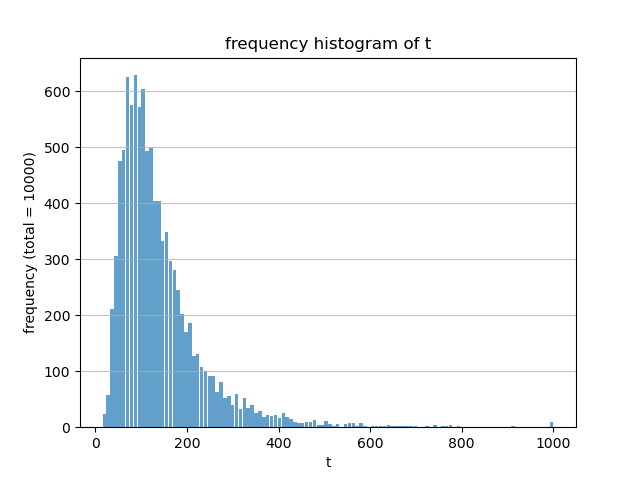
\includegraphics[width=5cm]{./fig/fig1_t.png}
}
\subfigure[$\log t$]{
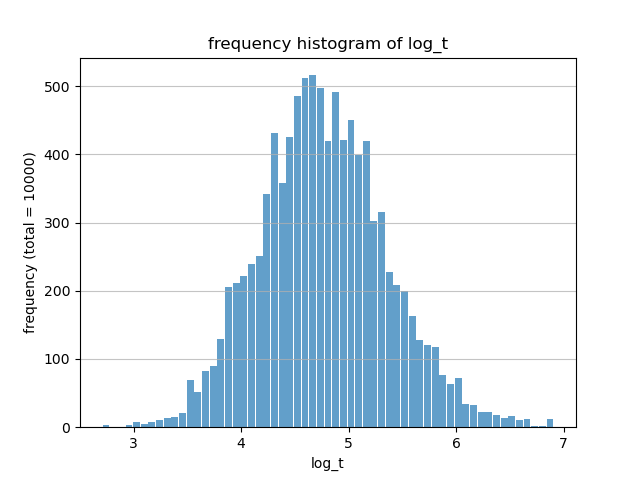
\includegraphics[width=5cm]{./fig/fig3_log_t.png}
}
\subfigure[$T$]{
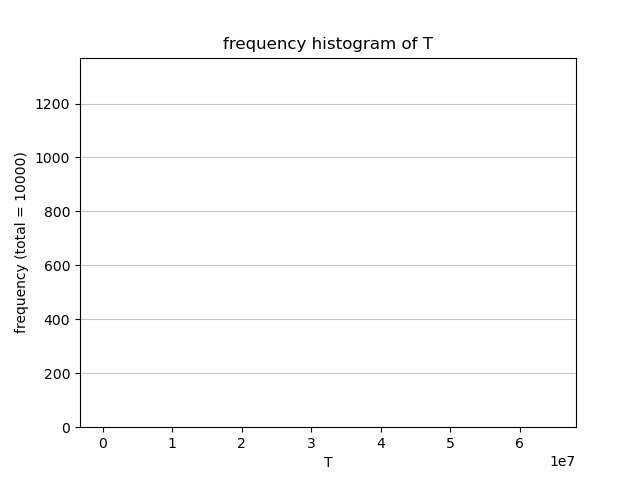
\includegraphics[width=5cm]{./fig/fig2_T.png}
}
\subfigure[$\log T$]{
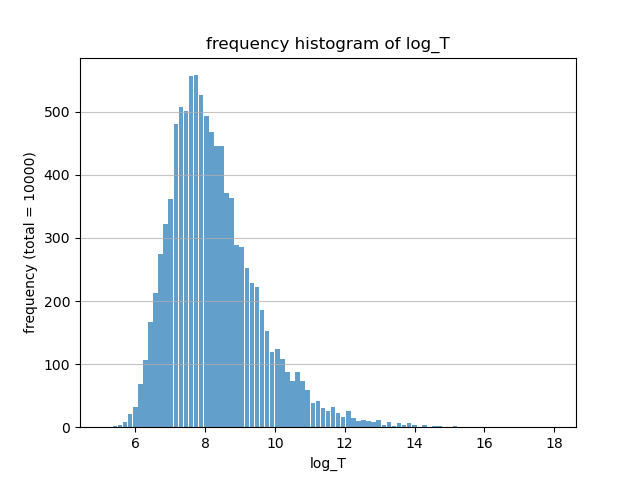
\includegraphics[width=5cm]{./fig/fig4_log_T.png}
}
\caption{$t$和$T$的直方图}\label{fig:hist}
\end{figure}

从图中可以看出:

$t$的分布主要在$[e^4,e^6]$,即$[55,403]$,平均值$141.14$。

$T$的分布主要在$[e^6,e^10]$,即$[403,22026]$,平均值$19512.07$。

大部分情况在平均值以下,仍然符合大约1\%的比例。但有少部分情况远远超出平均值,以至于不取对数就几乎看不到了。

\section{推广和总结}
\label{sec:extension}

\subsection{支持向量机}

对于线性可分的数据,在感知机中我们的目标仅仅是找到一个超平面能达到所有训练数据都能正常分类,而这个结果不唯一,其中任意一个都可能是算法的结果。看似这些结果的效果都相同,但机器学习方法最看中的并不是对于训练数据的判断能力,而是对未知数据的预测能力,也就是泛化能力。那么,怎样从中选择一个对未知数据效果最好的呢?

支持向量机给出的答案是:取以最大间隔把两个类分开的超平面,称为最佳超平面。如图\ref{fig:max margin}所示。

\begin{figure}[htbp]
\centering
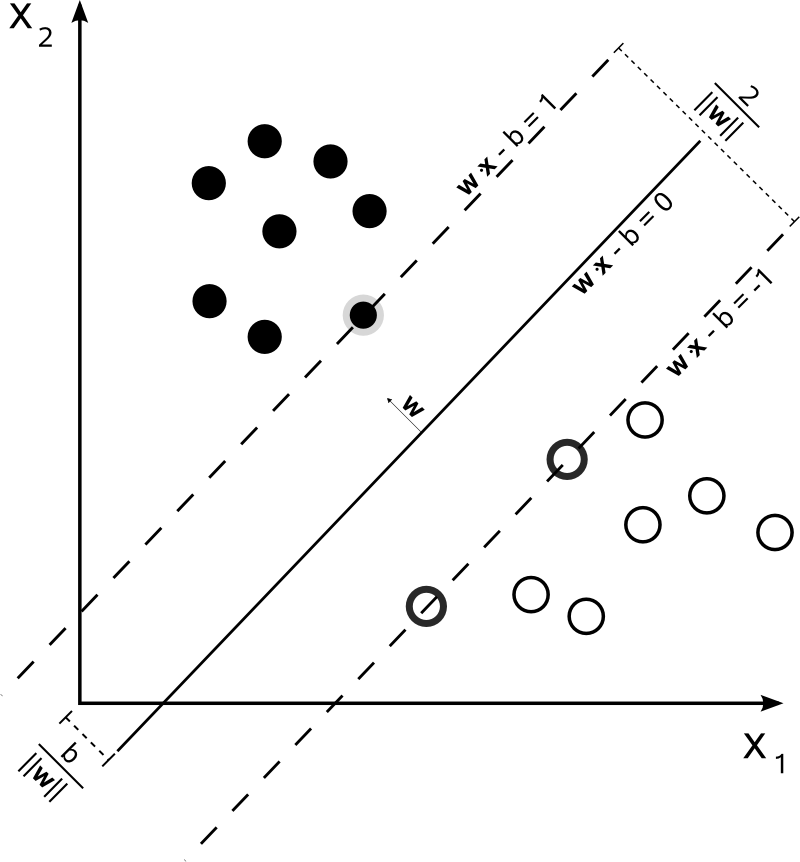
\includegraphics[width=6.5cm]{./fig/max_margin.png}
\caption{最佳超平面}\label{fig:max margin}
\end{figure}

其思路在图中表达的很清楚。

支持向量机的另一个优点是,他使用核方法(Kernel)在一定程度上解决了对于线性不可分数据的处理,如图\ref{fig:kernel}所示。

\begin{figure}[htbp]
\centering
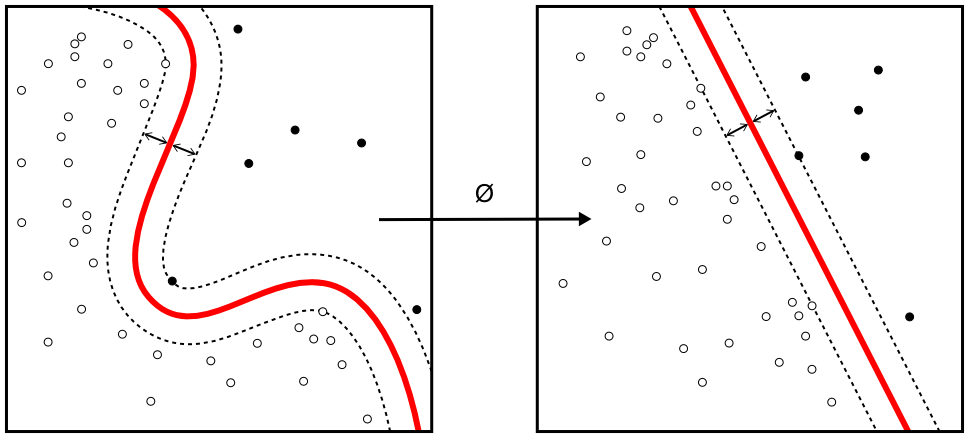
\includegraphics[width=10cm]{./fig/Kernel.png}
\caption{核方法}\label{fig:kernel}
\end{figure}

核方法的核心思想是:先通过某种非线性映射将原始数据嵌入到合适的高维特征空间,使其在高维特征空间是线性可分的,再利用已有的对线性可分数据的处理方法
在这个新的空间中分析和处理。

自从90年代初经典SVM的提出,由于其完整的理论框架和在实际应用中取得的很多好的效果,在机器学习领域受到了广泛的重视,其理论和应用在横向和纵向上都有了发展。

\subsection{神经网络和深度学习}

感知机模型一大缺点就是无法解决线性不可分问题,最经典的例子就是异或问题(XOR),如图\ref{fig:XOR}所示。
\begin{figure}[htbp]
\centering
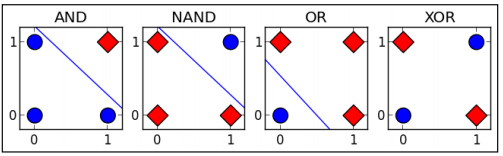
\includegraphics[width=10cm]{./fig/XOR.png}
\caption{异或(XOR)}\label{fig:XOR}
\end{figure}

对此,神经网络给出的答案是:将大量的人工神经元联结进行计算,构成“人工神经网络”,如图\ref{fig:net}所示。

\begin{figure}[htbp]
\centering
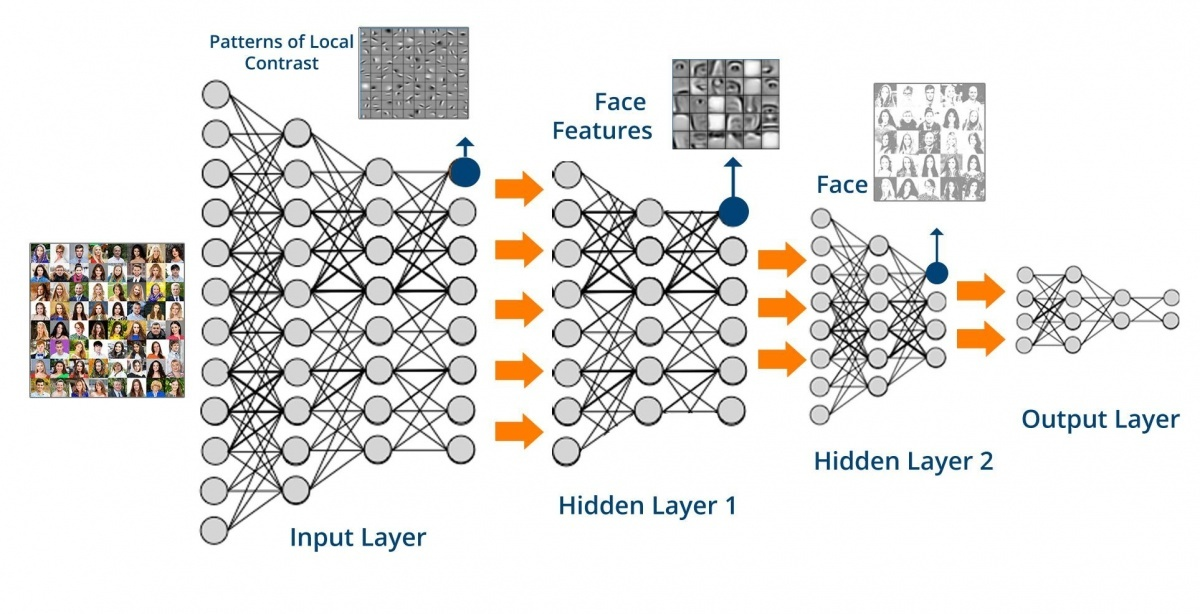
\includegraphics[width=10cm]{./fig/net.jpg}
\caption{多层神经网络}\label{fig:net}
\end{figure}

从神经网络的角度来看,感知机是一个最简单的单层神经网络,而神经网络的表现能力是随层数和每层的神经元数量增加而提高的。一个二层神经网络就可以对异或数据给出完美的分类方法,也就是实现了非线性。

深度学习可以简单的看成是大型神经网络,大主要体现在层数多,参数量大。其优点是表达能力极强,缺点是可能出现“过拟合”(如图\ref{fig:overfitting}),计算量巨大,对计算机硬件要求高。

\begin{figure}[htbp]
\centering
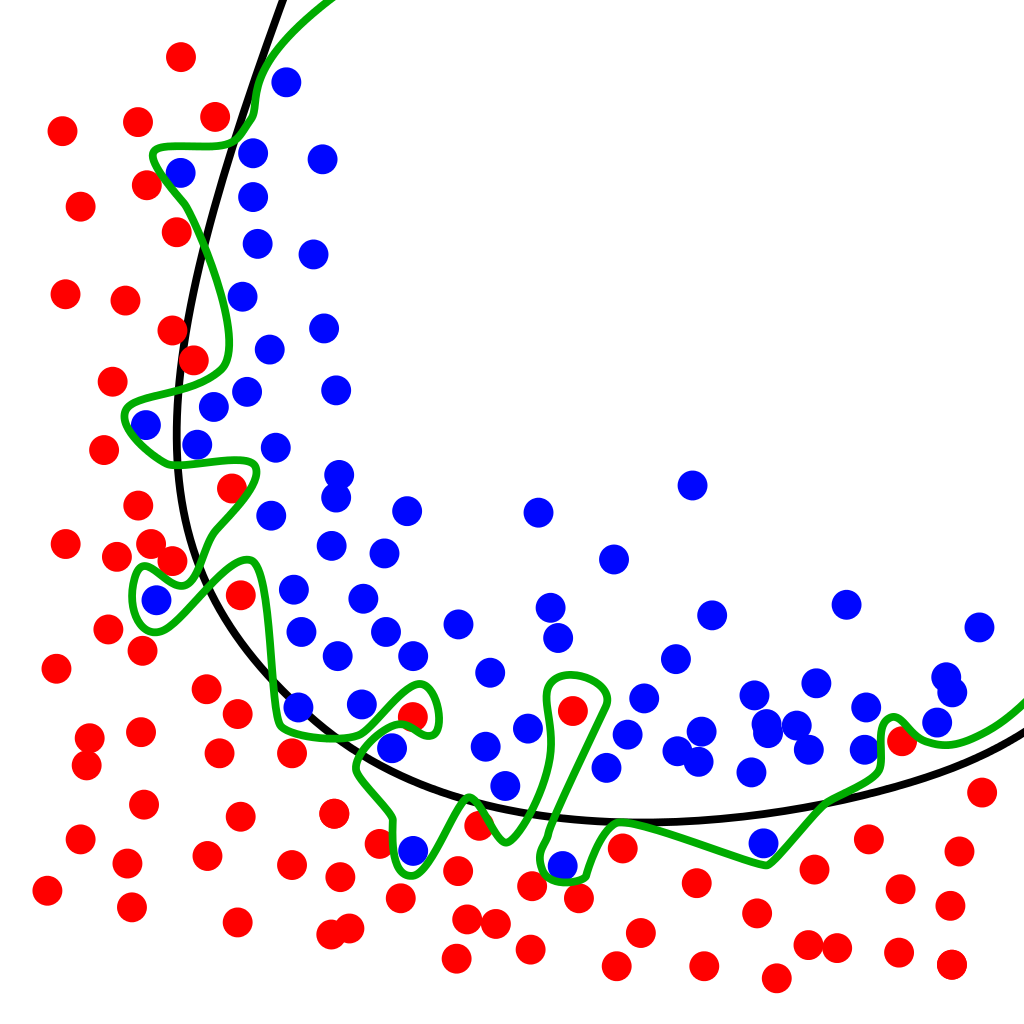
\includegraphics[width=6.5cm]{./fig/Overfitting.png}
\caption{绿线是过拟合的,黑线是泛化能力更好的}\label{fig:overfitting}
\end{figure}

从2006年开始,神经网络(第3代)发展迅速,目前神经网络和深度学习是人工智能领域最热门的研究方向,其应用(人脸识别,语音翻译,自动驾驶等)已经广泛应用到我们的日常生活中。

\subsection{总结}
从第\ref{sec:introduction}节的简介中我们知道,感知机也可以看作神经网络的最简单形式,而目前应用最广泛的人工智能技术“深度学习”的基础就是神经网络,因此我们也可以将感知机模型看作机器学习或深度学习的入门课。

现在如果提到感知机的优点,与支持向量机,神经网络等更高级的模型相比,基本上就只有“简单易行”了。但麻雀虽小五脏俱全,在这么简单的算法中我们学到了
目标函数的设计与简化,参数的迭代过程(随机梯度下降法),算法适用条件和收敛性分析。可以说是非常有教学意义了。


\appendix

\section{python程序}
\label{sec:pythoncode}
感知机库:Perceptron
\lstinputlisting[language=Python]{../perceptron.py}

运行demo
\lstinputlisting[language=Python]{../perceptron_demo.py}

\end{document}
